\chapter{Tecnologias Utilizadas}
\label{chap3}

\section{Neo4j}
O Neo4j é um sistema de gerenciamento de banco de dados orientado a grafos desenvolvido pela Neo4j Inc., que opera sob uma estrutura de dados que consiste em nós, relacionamentos e propriedades. Ao contrário dos bancos de dados relacionais, que usam tabelas e linhas, o Neo4j permite que as informações sejam armazenadas em um formato altamente conectado, imitando as interações do mundo real. Isso faz do Neo4j uma escolha ideal para cenários onde as relações entre os dados são tão importantes quanto os próprios dados.

 
Cada Nó e cada Aresta possui (faz parte de) um ou mais Rótulos (\textit{labels}), que instancia um index de lookup, funcionando similar à uma tabela num banco relacional. Podemos eficientemente recuperar os dados de todos os nós ou todas as arestas de um certo rótulo para listá-las, por exemplo.

Cada rótulo possui sua definição de \textit{tipo}, que define a tipagem de cada uma de suas propriedades, incluindo possíveis ligações com nós de mesmo, ou outro, rótulo.

\subsection{Cypher Query Language}
O banco Neo4j não utiliza SQL como a linguagem de manipulação de registros de dados, e sim uma linguagem própria chamada Cypher.

\begin{figure}[H]
    \centering
    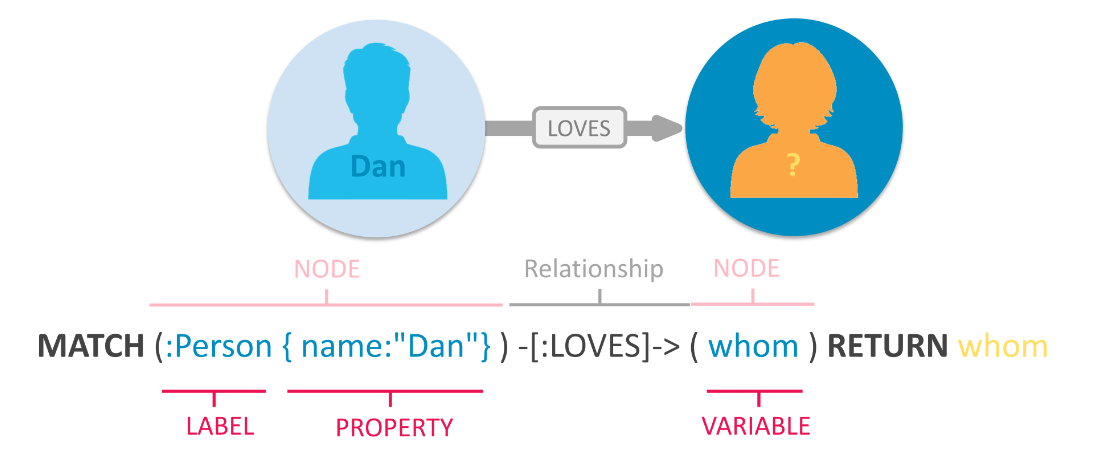
\includegraphics[width=1.0\linewidth]{Imagens/chap03/cypher-exemple.png}
    \caption{Exemplo de uma consulta em Cypher. Encontre os nós com \textit{rótulo} "\textit{Person}" (Pessoa) e propriedade "\textit{name}" (nome) igual à string "Dan", que também obrigatoriamente possui uma relação do \textit{tipo} "LOVES" ("AMA") com algum nó, salvar tais nós vizinhos em uma variável "whom" ("a quem"), e então retornar os dados contidos em "whom". Ou seja, \textit{retorne as pessoas que os "Dan"'s amam}. Imagem retirada de https://neo4j.com/developer/cypher/.}
    \label{fig:cypher-example}
\end{figure}
É através de Cyphers que ultimamente será feita a comunicação com os dados armazenados no Neo4j, porém a partir da interface e através das requisições em GraphQL, as bibliotecas no nosso servidor vão permitir gerármo-os automaticamente.

\section{GraphQL}

Optamos por utilizar uma API em GraphQL na comunicação entre a interface e o servidor. GraphQL é uma linguagem de consulta e manipulação de dados, que permite, em um único endpoint no servidor, escutar e resolver diferentes pedidos das interfaces clientes. O pedido é especificado através de uma linguagem chamada GraphQL (em arquivos .gql), que é enviada no corpo de uma requisições HTTP, sempre com verbo POST.

O servidor disponibiliza uma série de consultas e requisições de alterações (\textit{queries} e \textit{mutations}) para o cliente. Nessas operações, também é publicado quais são os seus argumentos e o \textit{tipo} de sua resposta.

O cliente então pode requisitar qualquer uma das funções disponíveis, e, da resposta, escolher exatamente o que precisa como retorno naquele momento. Tal escolha se dá através da estrutura em árvore da linguagem.

\subsection{@neo4j/graphql}
Para gerar todas as queries e mutations de CREATE READ UPDATE DELETE para os \textit{tipos} de nós e arestas disponíveis para o banco de dados, utilizamos 
a biblioteca oficial da neo4j que disponibiliza também linguagens para definir e gerar o schema do banco de dados.

Abaixo, vemos exemplos de possíveis pedidos em GraphQL enviados pelo cliente. Primeiro uma requisição para recuperar os alunos de uma certa escola, e as notas em suas provas.

\begin{lstlisting}
# .gql
query GetSchoolStudentsWithAssignmentGrades(schoolId: ID!){
    schools( where: {id: $schoolId}){
        students{
            id
            name
            assignments {
                id
                grade
            }
        }
    }
}
\end{lstlisting}

Se, além da nota (\textit{grade}) do aluno, o cliente precisar de uma descrição das provas (\textit{assignments}) dele, podemos apenas acrescentar tal propriedade na requisição. O mesmo pode ser feito com qualquer propriedade (incluindo arestas) definida no \textit{tipo}.

\begin{lstlisting}
            [...]
            assignments {
                id
                grade
                description
            }
            [...]
\end{lstlisting}
Andando pelas arestas (abrindo chaves) é possível retornar qualquer subconjunto de dados a partir do resultado da \textit{query} realizada (dado que é autorizado para tal), podemos requisitar exatamente o que o frontend precisa, minimizando os recursos de banda.

Segundo, um exemplo de requisição de operação de alteração (\textit{mutation}) na linguagem GraphQL.

\begin{lstlisting}
# .gql
mutation ChangeStudentEmail(id: ID! newEmail: string){
    updateStudent(
        where: {id: $id}, 
        update: {email: newEmail}
    ){
        student {
            id
        }
    }
}
\end{lstlisting}

Tais requisições seriam resolvidas quando eviadas à um servidor no qual utilizamos a biblioteca @neo4j/graphql com as definições de \textit{tipos} simplificadas como a seguir:

\begin{lstlisting}
# types.graphql
type School{
    id: ID
    students: [Student]	@relationship
    [...]
}

type Student {
    id: ID
    assignments [Assignment] @relationship
    [...]
}

type Assignment {
    id: ID
    grade: Float
    description: String
    [...]
}
\end{lstlisting}


\section{Apollo}

Biblioteca de gerenciamento de estados para JavaScript, através de GraphQL. É composta pois duas partes que se comunicam entre si:
\begin{itemize}
    \item \textbf{Apollo Client} - Utilizado na aplicação cliente. Permite funcionalidade de controle de requisição de dados, variáveis de carregamento, controle de cache, e variáveis de estados locais. Auxilia o processo de realizar requisições em GraphQL.
    \item \textbf{Apollo Server} - Servidor GraphQL compatível com qualquer cliente que envia uma requisição GraphQL à ele, incluindo Apollo Clients. Utilizado na geração do schema que as requisições (e consequentemente os dados) precisam seguir. É conectado com poder de gerenciamento à qualquer fonte de dados (no caso do projeto do trabalho, um banco Neo4j).

\end{itemize}

\section{Node.js}

Software de código aberto baseado no interpretador V8 que permite a execução de códigos JavaScript em múltiplas plataformas.

\section{Express.js}

Framework web mais popular para node.js. Minimalista,  disponibilizando apenas funcionalidades básicas para desenvolvimento web como handling para diferentes verbos HTTP, e, crucialmente para o projeto, middlewares para camadas de autenticação e autorização.


\begin{lstlisting}
const express = require("express");
const app = express();
const port = 3000;

app.use(function (req, res, next) {
    if (!isRequestAllowed(req)) {
        return res.status(403).send({
            message: "You don't have permissions to execute this request.",
        });
    }
    return next();
});
// app.get("/", function(req,res) {...});
// app.post("/example", ...);

app.listen(port, function () {
  console.log(`Escutando na porta ${port}!`);
});
\end{lstlisting}
\section{Vue.js}

Vue.js é um framework para construir interfaces web. Disponibiliza um processo intuitivo de desenvolvimento de componentes e telas reativas. Os arquivos .vue contém três partes:
\begin{itemize}
    \item o \textbf{Template} em HTML que serve para organizar os componentes na tela, com interação direta com o JavaScript através das diretivas lógicas como v-for (permitindo renderização iterativa de componentes), v-if (permitindo renderização condicional), v-model (que permite criar ligações bidirecionais entre variáveis em diferentes componentes) dentre outras.
    \item o \textbf{Script}, que abriga as funcionalidades lógicas do componente, incluindo requisições ao banco de dados e controle de estados da interface
    \item o \textbf{Style}, onde estão as regras de CSS que ditam os estilos dos componentes
\end{itemize}
